% Chapter 6

\chapter{RESULTS AND DISCUSSION} % Write in your own chapter title

\section{DATASET FOR TESTING} 
The input to the system is the Ling Spam PU1 Corpus. The dataset is divided into 10 subdirectories (part1, part2…part10), each of which contains 241 ham messages and 48 spam messages. The subdirectories correspond to the 10 fold validation experiments, where 9 parts are used for training and 1 part is used for testing.  The results of this module testing as well as the testing of the entire system are summarized below. 

\section{OUTPUT OBTAINED IN VARIOUS STAGES} 
This section shows the results obtained during module testing.

\subsection{INPUT}
Part 10 of the dataset is considered as the input to the system. It contains 241 ham messages and 48 spam messages. Figure 6.1 depicts the input.

\subsection{TOKENIZING AND STOP WORD REMOVAL}
The output of Tokenization and Stop Word removal is shown in figure 6.2.

\subsection{TF-IDF VECTORIZATION}
Figure 6.3 shows the output of the TF-IDF vectorizer.

\subsection{SINGULAR VALUE DECOMPOSITION}
The output of the SVD stage is shown in figure 6.4. The matrices U, S and V are also depicted.

%\subsection{MODIFIED INDEXING}


\section{SAMPLE SCREENSHOTS DURING TESTING}


The screen shot is shown in Figure 6.1 for better reference.

\begin{figure*}[h]
\centering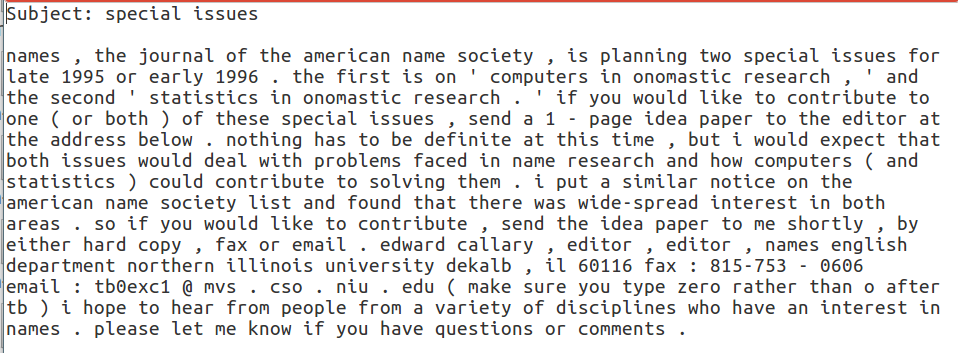
\includegraphics[width=1.0\linewidth]{email.png}
\caption{Screenshot of an email}
\end{figure}

An example of the term by document matrix is show in Figure 6.2.

\begin{figure*}[h]
\centering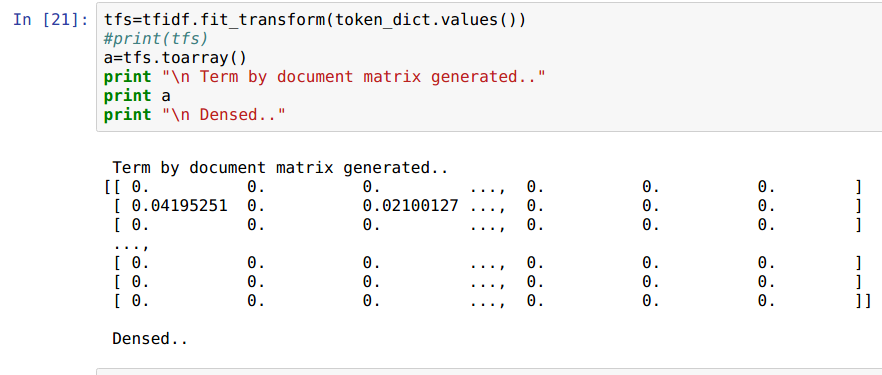
\includegraphics[width=1.0\linewidth]{term.png}
\caption{Screenshot of Term of Document Matrix}
\end{figure}

An example of the single value decomposition is shown in Figure 6.3.

\begin{figure*}[h]
\centering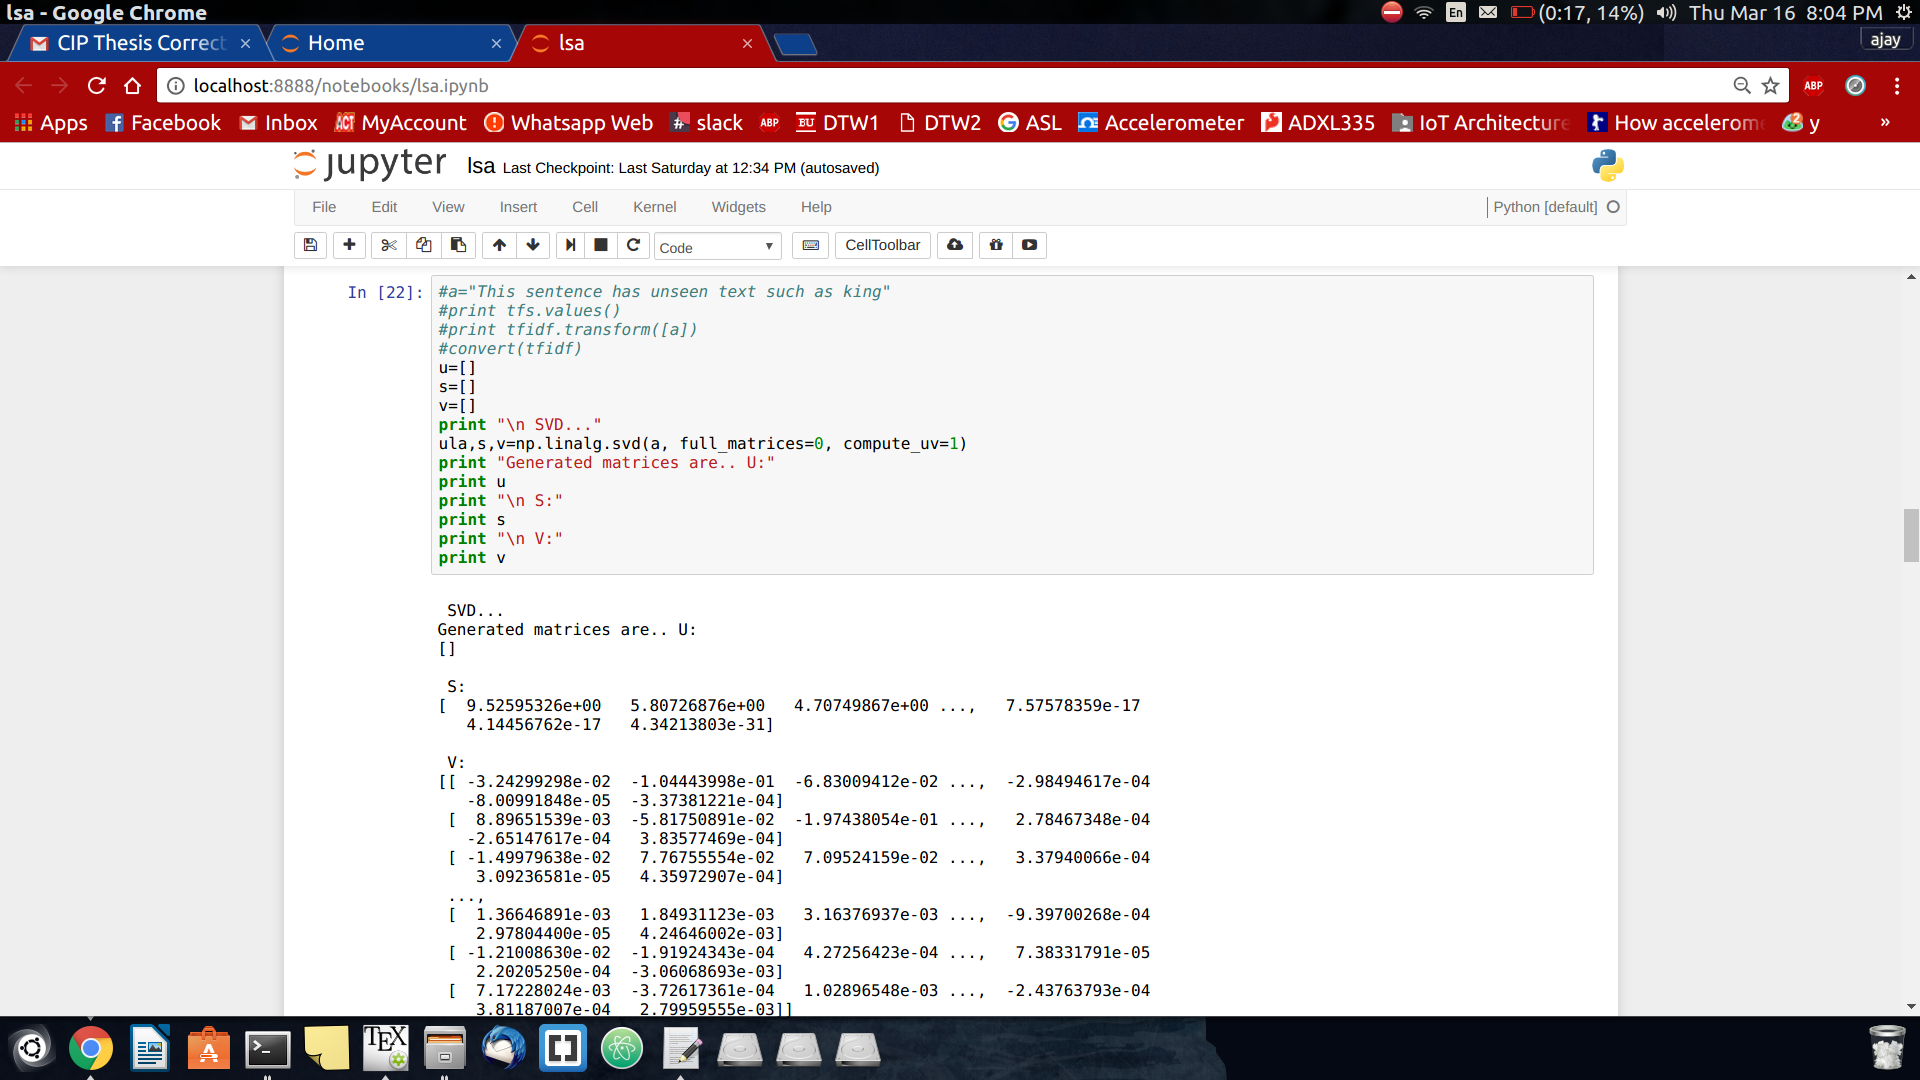
\includegraphics[width=1.0\linewidth]{svd.png}
\caption{Screenshot of SVD}
\end{figure}

The system is tested for various test cases which are detailed in Appendix A module-wise.

\textbf{wecol ' 98 
- - western conference on linguistics
arizona state university cordially invites you to attend wecol ' 98 ( western conference on linguistics ) , to be held in conjunction with lasso xxvii , 9-11 october 1998 . information about the conference ( s ) may be found at our websites : http : / / www . public . asu . edu / ~ teresalw / wecol . htm http : / / www . public . asu . edu / ~ teresalw / lasso . htm these sites include preliminary programs as well as information about the meeting site , lodging , nearby areas of interest , and your host institution arizona state university . please feel free to contact the pagemaster of the site , teresa . wells @ asu . edu , with any questions . teresa wells research assistant to dr . elly van gelderen english department arizona state university} 


The training of the neural network using the corpus is shown in Figure 6.4.

\begin{figure*}[h]
\centering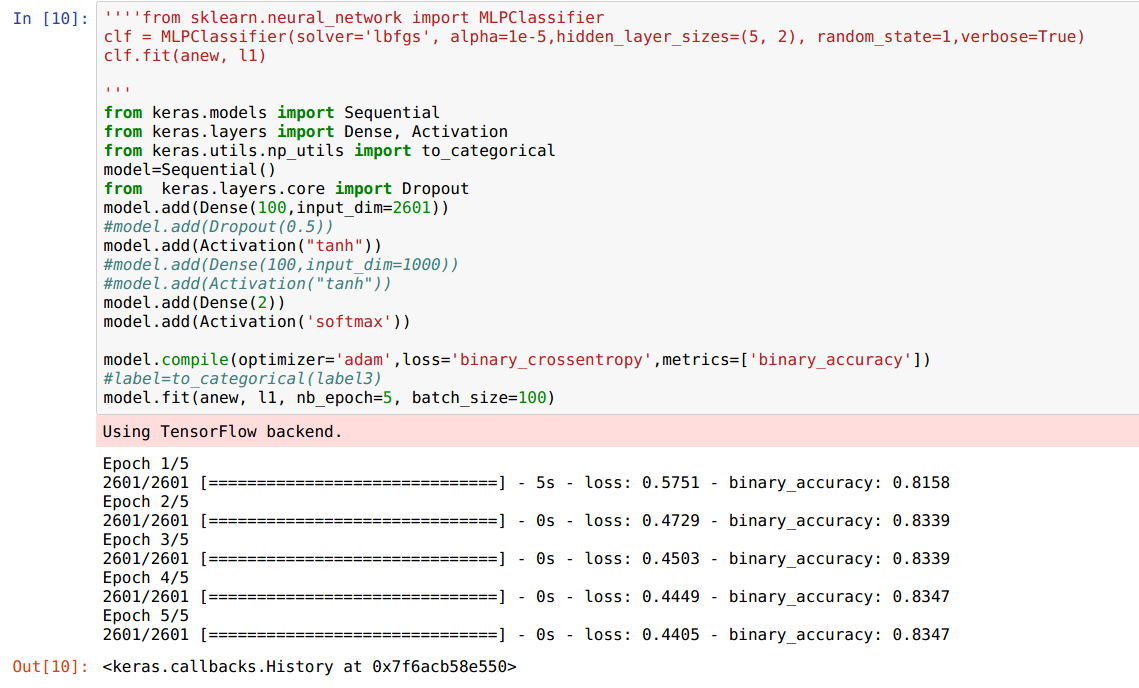
\includegraphics[width=1.0\linewidth]{net.png}
\caption{Screenshot of training}
\end{figure}

\section{PERFORMANCE EVALUATION}
The performance of the entire system is evaluated using the standard parameters described below. 
\subsection{PRECISION}
\subsubsection{DESCRIPTION}
Precision refers to the fraction of retrieved instances that are relevant. It is a measure of exactness i.e what \% of tuples that the classifier labeled as positive is actually positive. It is calculated as the number of true positives (Tp) over the number of true positives plus the number of false positives (Fp). Precision always ranges from 0 to 1, with higher values indicating better classification. Precision is calculated by equation 6.1 as:


$Precision=TP/(TP+FP)$


TP is the number of actual ham messages classified correctly


FP is the number of actual spam messages misclassified as ham


\subsubsection{ALGORITHM}
The algorithm to calculate precision is as follows:


Find the total number of true positives i.e actual ham messages being correctly classified as ham (TP).


Find the number of false positives i.e actual spam messages being classified incorrectly as ham (FP).


Substitute TP and FP values in equation 6.1 to obtain precision.


\subsection{RECALL}
\subsubsection{DESCRIPTION}
Recall refers to the fraction of relevant instances that are retrieved. It is a measure of completeness i.e what \% of positive tuples did the classifier label as positive. It is calculated as the number of true positives (Tp) over the number of true positives plus the number of false negatives (Fn). Recall also ranges from 0 to 1, with 1.0 being considered as the perfect score. Recall is calculated using equation as:


$Recall=TP/(TP+FP)$


TP is the number of ham messages classified correctly


FN is the number of ham messages misclassified as spam


\subsubsection{ALGORITHM}
The algorithm to calculate recall is as follows


Find the total number of true positives i.e actual ham messages being correctly classified as ham (TP).


Find the number of false negatives i.e actual ham messages being classified incorrectly as spam (FN).


Substitute TP and FP values in equation 6.2 to obtain precision.

\subsection{F-MEASURE}
\subsubsection{DESCRIPTION}
F measure (or F1 Score) is the harmonic mean of precision and recall. It varies from 0 to 1, with higher values considered better. F measure is calculated by equation 6.3 as:


$F-Measure=2TP/(2TP+FP+FN)$


TP is the number of ham messages classified correctly


FP is the number of spam messages incorrectly classified as ham


FN is the number of ham messages misclassified as spam


\subsubsection{ALGORITHM}
The algorithm to calculate the F measure is as follows:


Find the total number of true positives i.e actual ham messages being correctly 
classified as ham (TP).


Find the number of false positives i.e actual spam messages being classified incorrectly as ham (FP).


Find the number of false negatives i.e actual ham messages being classified incorrectly as spam (FN).


Substitute TP, FP and FN values in equation 6.3 to obtain precision.


\subsection{ACCURACY}
Accuracy is defined as the ratio of the True Positives and True Negatives to the entire classified dataset.


$Accuracy=(TP+TP)/(TP+FP+TN+FN)$


The major disadvantage of this metric is that for a biased dataset, even a trivial classifier – one that classifies all test data as only spam/ham is likely to give an appreciable value. Therefore, F measure is generally considered as a better evaluation metric.


\section{SCORES OBTAINED AND DISCUSSION}}
Table 6.1 shows the distribution of our test set. The first row contains the True Positive (TP) and False Negative (FN) values respectively. The second row contains False Positive (FP) and True Negative (TN) values respectively.


\begin{table}[ht]
\centering
\caption{Overall Classification of a test-batch}
\label{my-label}
\begin{tabular}{|l|l|l|}
\hline
\textit{\textbf{Overall Classification}} & \textbf{Positive} & \textbf{Negative} \\ \hline
\textit{\textbf{Positive}}               & 203               & 38                \\ \hline
\textit{\textbf{Negative}}               & 37                & 10                \\ \hline
\end{tabular}
\end{table}
\\
$Precision=(203/(203+37))=0.8458$
\\
$Recall=(203/(203+38))=0.8423$
\\
$F-Measure=((2+203)/(2+203+37+38))=0.844$
\\
$Accuracy=((203+10)/(203+37+38+10))=0.7473$
%\begin{figure}[h]
%\centering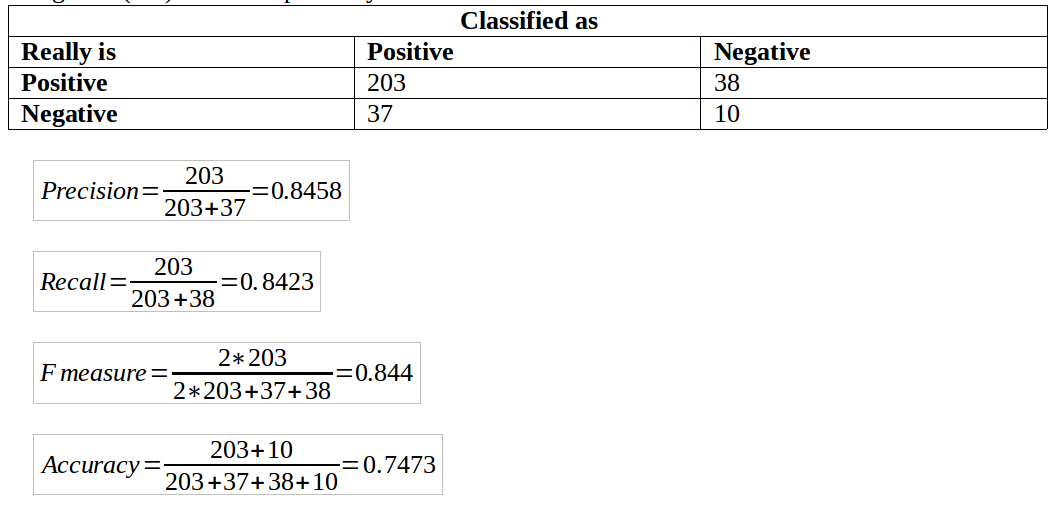
\includegraphics[width=0.8\linewidth]{score.png}
%\caption{Score wise analysis}
%\end{figure}


\section{DOMAIN WISE ANALYSIS}
The test dataset contains data related to three main domains – Personal, Work and Academia. Table 6.2 shows the classification split up of the different domains. Using the formulae mentioned above, the domain-wise metrics can be obtained.

%\begin{tabular}{|l|l|l|l|l|l|l|}
%\hline
%        & personal      & work          & acadamics     \\
%\hline
% Actual & Classified as & Classified as & Classified as \\
%\hline
%        & p             & n             & p             \\
%\hline
% p      & 68            & 12            & 67            \\
%\hline
% n      & 11            & 0             & 12            \\
%\hline
%\end{tabular}

\begin{table}[]
\centering
\caption{Personal Domain -Spam classification of personal mails}
\label{my-label}
\begin{tabular}{|l|l|l|}
\hline
\textit{\textbf{Personal}} & Positive & Negative \\ \hline
Positive                   & 68       & 12       \\ \hline
Negative                   & 11       & 0        \\ \hline
\end{tabular}
\end{table}

\begin{table}[]
\centering
\caption{Work Domain -Spam classification of work mails}
\label{my-label}
\begin{tabular}{|l|l|l|}
\hline
\textit{\textbf{Work}} & Positive & Negative \\ \hline
Positive                   & 67       & 13       \\ \hline
Negative                   & 12       & 5        \\ \hline
\end{tabular}
\end{table}

\begin{table}[]
\centering
\caption{Academia Domain -Spam classification of academia mails}
\label{my-label}
\begin{tabular}{|l|l|l|}
\hline
\textit{\textbf{Academia}} & Positive & Negative \\ \hline
Positive                   & 68       & 13       \\ \hline
Negative                   & 14       & 5        \\ \hline
\end{tabular}
\end{table}

%\begin{figure}[h]
%\centering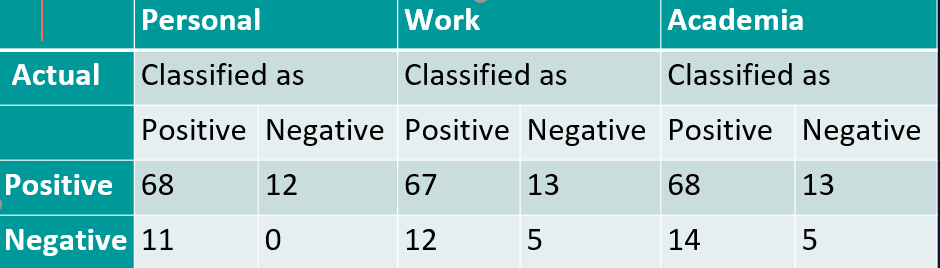
\includegraphics[width=0.8\linewidth]{table.PNG}
%\caption{Domain Wise Analysis}
%\end{figure}


The domain wise distribution of evaluation metrics is shown below.


\begin{figure}[h]
\centering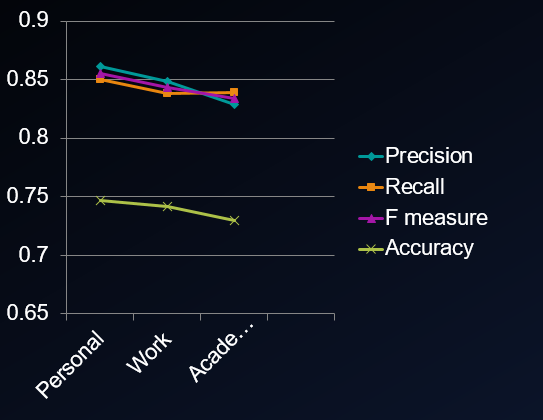
\includegraphics[width=0.5\linewidth]{graph1.PNG}
\caption{Domain Wise Analysis(a)}
\end{figure}
\begin{figure}[h]
\centering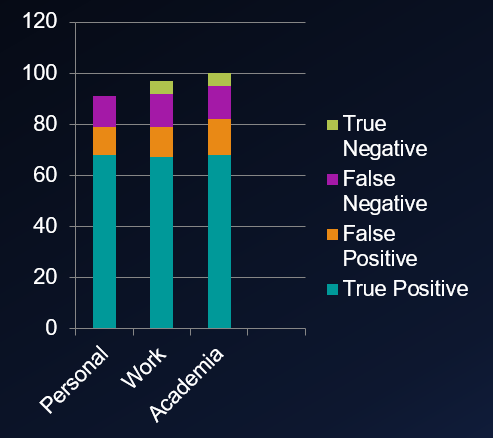
\includegraphics[width=0.5\linewidth]{graph2.PNG}
\caption{Domain Wise Analysis(b)}
\end{figure}
